% ******************************* Thesis Appendix C ********************************

\chapter{Detalles adicionales sobre pruebas realizadas}
\label{appendix6}

% **************************** Define Graphics Path **************************
\ifpdf
    \graphicspath{{Appendix6/Figs/Raster/}{Appendix6/Figs/PDF/}{Appendix6/Figs/}}
\else
    \graphicspath{{Appendix6/Figs/Vector/}{Appendix6/Figs/}}
\fi

En el presente anexo se incluyen detalles t\'ecnicos acerca de las pruebas realizadas sobre el Laboratorio de experimentaci\'on con el fin de validar el prototipo. El mismo esta dividido en secciones complementarias a diferentes secciones del cap\'itulo 6; por ello se recomienda leer primero la correspondiente secci\'on en el cap\'itulo 6 y luego complementar la lectura con este cap\'itulo.

\section{Escenario 1 - Algoritmo de Ruteo}
\label{appendix6.1}
En las figuras ~\ref{fig:CU1P1DumpFlows1}~-~\ref{fig:CU1P1DumpFlows4} se muestran las tablas de flujos asociadas a cada nodo del laboratorio. Para conseguir esta informaci\'on se utiliza el comando \textbf{dump-flows} de la herramienta Open vSwitch. Sin embargo puede obtenerse tambi\'en esta informaci\'on desde la propia interfaz gr\'afica de RAUFlow.\\

\newpage
\begin{figure}[ht!] 
\centering    
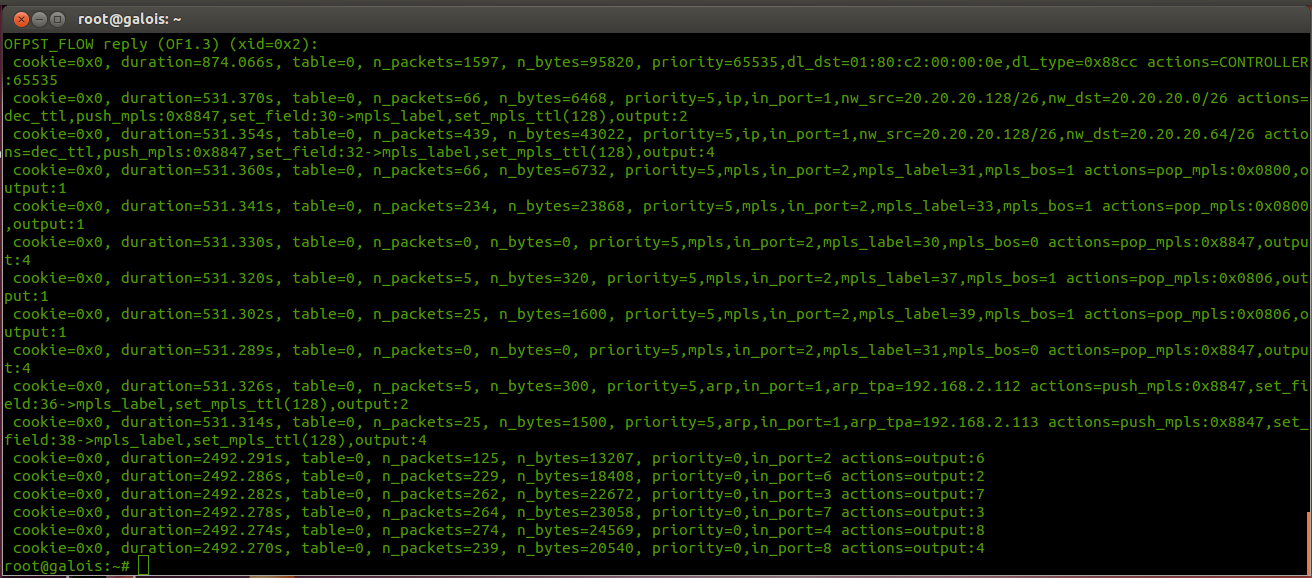
\includegraphics[width=1.0\textwidth]{E1P1/LabE1P1Gal}
\caption[Tabla de flujos ovs - Galois]{Tabla de flujos ovs - Galois}
\label{fig:CU1P1DumpFlows1}
\end{figure}

\begin{figure}[h!] 
\centering    
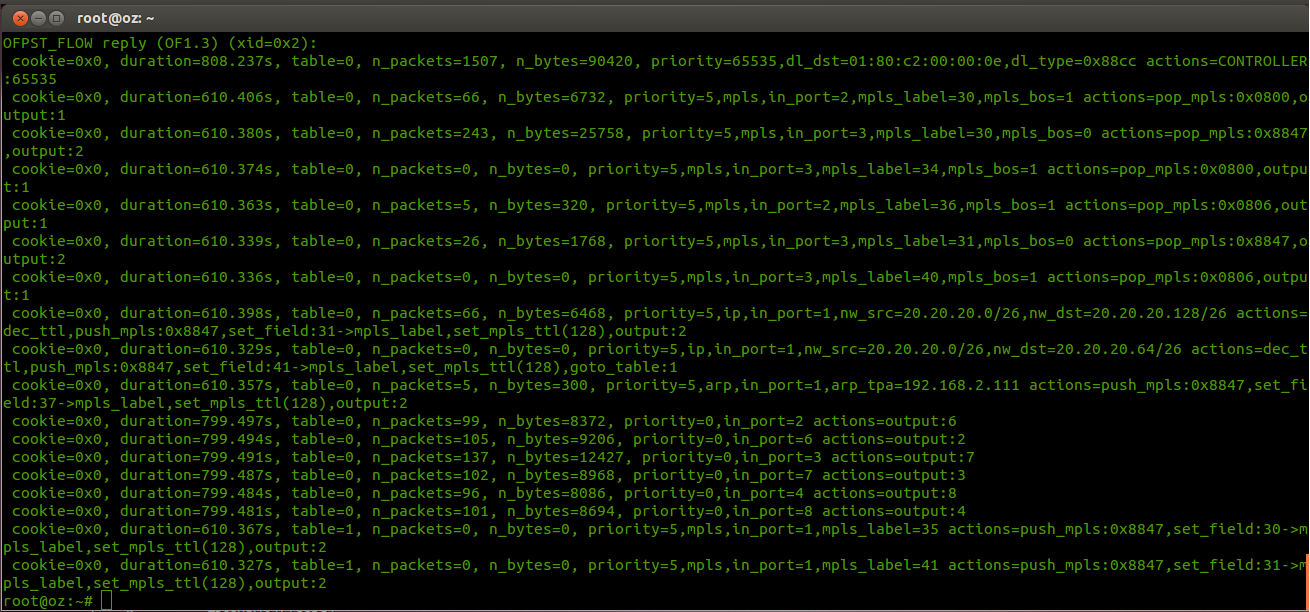
\includegraphics[width=1.0\textwidth]{E1P1/LabE1P1Oz}
\caption[Tabla de flujos ovs - Oz]{Tabla de flujos ovs - Oz}
\label{fig:CU1P1DumpFlows2}
\end{figure}

\begin{figure}[h!] 
\centering    
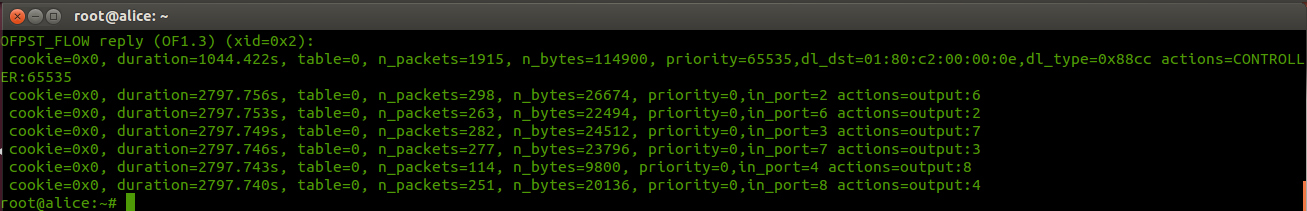
\includegraphics[width=1.0\textwidth]{E1P1/LabE1P1Al}
\caption[Tabla de flujos ovs - Alice]{Tabla de flujos ovs - Alice}
\label{fig:CU1P1DumpFlows3}
\end{figure}

\begin{figure}[h!] 
\centering    
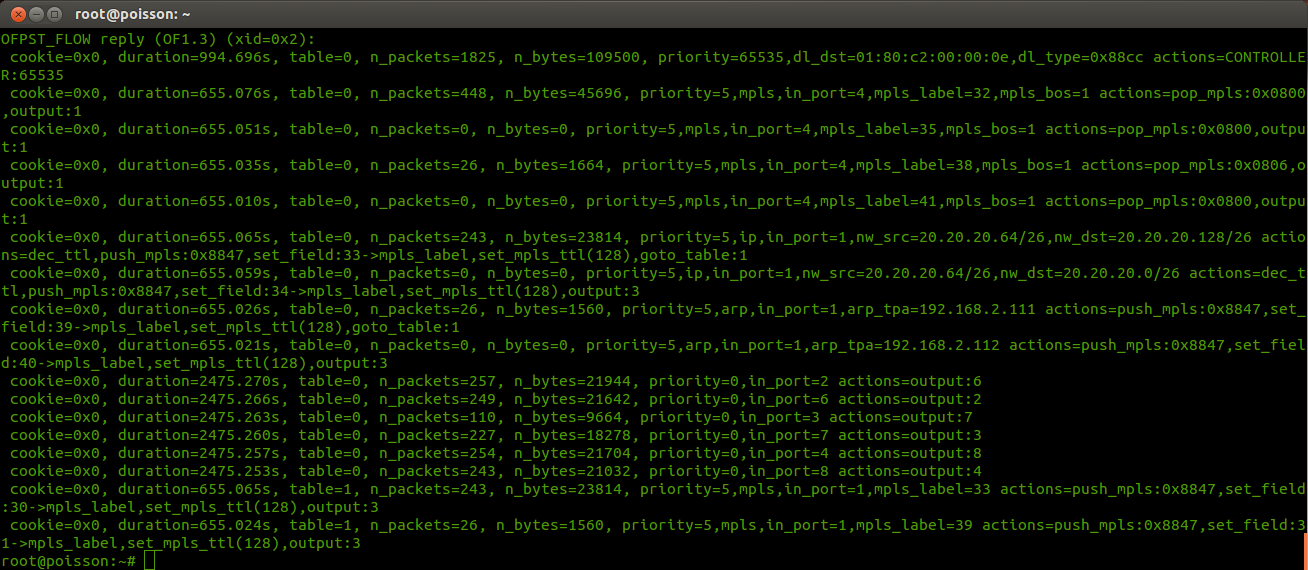
\includegraphics[width=1.0\textwidth]{E1P1/LabE1P1Poi}
\caption[Tabla de flujos ovs - Poisson]{Tabla de flujos ovs - Poisson}
\label{fig:CU1P1DumpFlows4}
\end{figure}

\newpage
Asumiéndose la notaci\'on $(n, i)$ para referirse a un enlace, donde \textit{n} indica nodo origen e \textit{i} interfaz de reenvío en \textit{n} para el próximo salto, entonces $<(n_1, i_1), \dots, (n_k, i_k)>$ puede usarse para denotar un camino en el laboratorio. De esta forma se pueden comparar f\'acilmente los caminos te\'oricos con los calculados.\\

Tomando como ejemplo el caso del servicio S3, el camino te\'orico puede denotarse de la siguiente forma:
 
$$<(Galois, nf_2)>$$

En otras palabras todo tr\'afico IP con origen en la subred A y destino a la subred B, es encaminado a través de la interfaz $nf_2$ en el nodo de ingreso \textit{Galois}. Luego en el nodo de egreso \textit{Poisson} es reenviado por la correspondiente interfaz del servicio.\\

Analizando las tablas de flujos de los nodos \textit{Galois} y \textit{Poisson}, puede comprobarse fácilmente la correspondencia entre el camino calculado y el camino te\'orico.

Por un lado en la tabla de flujos del nodo \textit{Galois} se tiene el siguiente flujo:

%Por un lado, acorde a la definci\'on del servicio, Galois debería reenviar todo tr\'afico de tipo \textbf{ip} que ingresa por la interfaz eth1(la cual se corresponde con el n\'umero de puerto openflow 1), con origen en la subred 20.20.20.64/26 y destino 20.20.20.0/64 por la interfaz nf1(la cual se corresponde con el n\'umero de puerto openflow 3).

\begin{figure}[h]
\textit{cookie=0.0, duration=531.354s, table=0, n\_packets=0, n\_bytes=0, priority=5, \\
ip,in\_port=1, nw\_src=20.20.20.128/26,nw\_dst=20.20.20.0/26 \\
actions=dec\_ttl,push\_mpls:0x8847,set\_field:30->mpls\_label,set\_mpls\_ttl(128),output:4}
\centering
\caption{Flujo 1}
\label{fig:Flujo1}
\end{figure}

Este flujo toma todo paquete recibido por el puerto openflow identificado con el n\'umero 1 (interfaz eth1), numeración IP origen 20.20.20.128/26 (subred A) y destino 20.20.20.64/26 (subred B), decrementa el TTL del paquete, coloca un cabezal mpls con la etiqueta 32 y finalmente lo reenvía por el puerto openflow identificado con el n\'umero 4 (interfaz nf2). Observar que el valor de la etiqueta mpls colocado es el utilizado para identificar el servicio (etiqueta interna). \\

%Notese adem\'as la acci\'on \textbf{dec\_ttl} en el flujo. Esta acci\'on es utilizada en cada nodo de borde en la definici\'on de un servicio para decrementar el ttl de un paquete ip cada vez que ingresa a la red del prototipo (en este caso a la red del laboratorio). Observese tambi\'en el valor de la etiqueta mpls(34) colocado en el paquete para identificar el servicio(etiqueta interna).

El procesamiento de los paquetes asociados al servicio S3 en el nodo \textit{Poisson}, esta dado por el siguiente flujo:

\begin{figure}[h]
\textit{cookie=0.0, duration=655.076s, table=0, n\_packets=0, n\_bytes=0, priority=5, \\
mpls,in\_port=4,mpls\_label=32,mpls\_bos=1 \\
actions=pop\_mpls:0x0800,output:1 }
\centering
\caption{Flujo 2}
\label{fig:Flujo2}
\end{figure}

Este flujo toma todo paquete recibido por el puerto openflow n\'umero 4 (interfaz nf2), retira el cabezal mpls y finalmente lo reenvía por el puerto n\'umero 1 (interfaz eth1).\\

De esta forma todos los paquetes asociados al servicio S3 son transportados desde el nodo de ingreso \textit{Galois} al nodo de egreso \textit{Poisson} mediante un solo enlace, utilizando un solo nivel de etiquetas mpls.\\

Analizando el camino que deben seguir los paquetes que atraviesan la red del laboratorio en el sentido inverso; es decir, desde la subred B hacia la subred A (servicio S4), el camino teórico es el siguiente:

$$<(Poisson, nf_1), (Oz, nf_0)>$$ 

Analizando primero la tabla de flujos del nodo \textit{Poisson}, el primer salto del camino es implementado por los siguientes flujos:

\begin{center}
\textit{cookie=0.0, duration=655.065s, table=0, n\_packets=0, n\_bytes=0, priority=5, \\
ip,in\_port=1, nw\_src=20.20.20.64/26,nw\_dst=20.20.20.128/26 \\
actions=dec\_ttl,push\_mpls:0x8847,set\_field:33->mpls\_label,set\_mpls\_ttl (128), goto\_table:1 \\
cookie=0.0, duration=655.065s, table=0, n\_packets=0, n\_bytes=0, priority=5, \\
mpls,in\_port=1,mpls\_label=33 actions=push\_mpls:0x8847,set\_fied:30->mpls\_label,set\_mpls\_ttl(128),output:3
}
\end{center}

Notar como primera diferencia en comparación al camino anterior, en este caso se tienen dos flujos: un primer flujo para colocar la etiqueta asociada al servicio (etiqueta interna) y un segundo flujo para colocar la etiqueta de reenvío (etiqueta externa). 

El camino anterior carece de etiqueta externa puesto que al ser un camino de un solo salto, el primer nodo coincide con el pen\'ultimo, y al implementar PHP no es necesario colocar etiqueta externa. 

Tras colocar el par de etiquetas mpls sobre el paquete al ingreso, el mismo es reenviado a trav\'es del puerto n\'umero 3 (interfaz nf1).\\

El siguiente salto en el camino, es implementado por el siguiente flujo en la tabla del nodo \textit{Oz}:

\begin{center}
\textit{cookie=0.0, duration=610.380s, table=0, n\_packets=243, n\_bytes=25748, priority=5, \\
mpls,in\_port=3,mpls\_label=30,mpls\_bos=0 actions=pop\_mpls:0x8847,output:2 }
\end{center}

Tras ingresar un paquete, se cambia el valor de la etiqueta externa para luego reenviarse por el puerto n\'umero 4 (interfaz nf2).\\

Luego el tramo final del camino es implementado en el nodo \textit{Galois} mediante el siguiente flujo:

\begin{center}
\textit{cookie=0.0, duration=531.341s, table=0, n\_packets=234, n\_bytes=23868, priority=5, \\
mpls,in\_port=2,mpls\_label=33,mpls\_bos=1 actions=pop\_mpls:0x0800,output:1 }
\end{center}

Análogamente el lector puede completar el análisis de la correspondencia entre los caminos te\'oricos y los calculados por el algoritmo de ruteo. A continuaci\'on se analiza la clasificaci\'on de tr\'afico.

\section{Escenario 1 - Clasificación de tr\'afico}
\label{appendix6.2}

\begin{figure}[ht!] 
\centering    
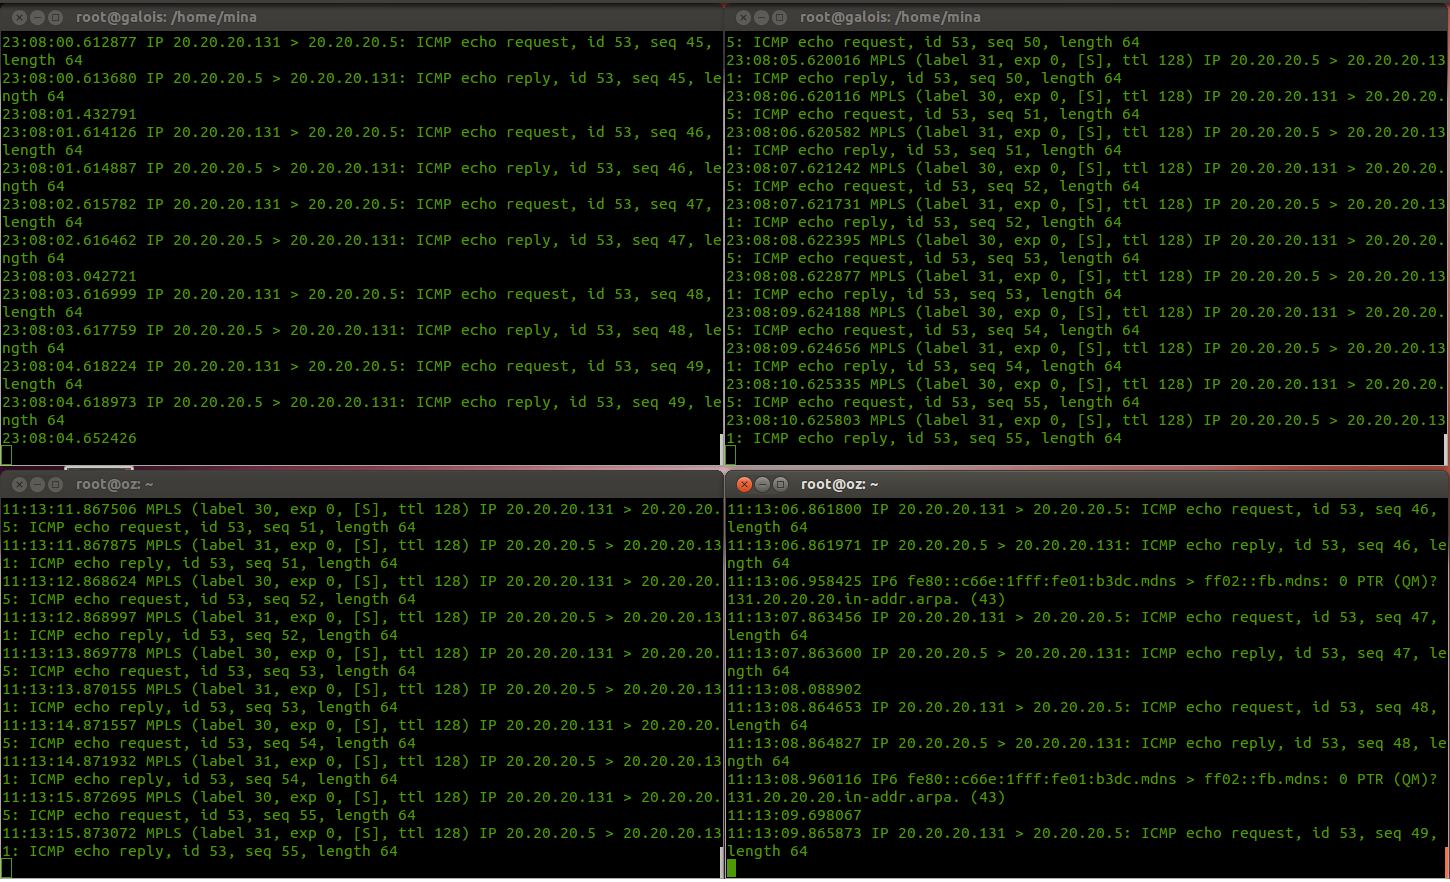
\includegraphics[width=1.0\textwidth]{E1P1/LabE1P1CaputrasTrafico0}
\caption[Capturas de tr\'afico con tcpdump - servicio S1]{Capturas de tr\'afico con tcpdump - servicio S1}
\label{fig:LabE1P1CapsTraf}
\end{figure}

En la figura \ref{fig:LabE1P1CapsTraf} se muestra el procesamiento de los paquetes asociados al servicio S1 en cada uno de los nodos que componen al LSP, generando tr\'afico desde un host en la sub red A con destino a otro host en la subred C.

Como puede observarse en el primer cuarto de la imagen (cuarto superior izquierdo), el cual se corresponde con una captura hecha con el comando \textbf{tcpdump} en la interfaz \textbf{eth1} del nodo \textit{Galois}, se reciben paquetes ICMP request con origen 20.20.20.131 y destino 20.20.20.05. Tambi\'en puede observarse en esta imagen paquetes ICMP reply a los paquetes request enviados.

Luego, como se muestra en el segundo cuarto de la imagen (cuarto superior derecho), el cual se corresponde con una captura realizada en la interfaz nf0 de dicho nodo, a cada paquete ICMP request recibido por la interfaz eth1 se le coloca un cabezal mpls con la etiqueta 31 y se reenvía por la interfaz en cuestión. Finalmente al arribar al nodo \textit{Oz} por la interfaz \textbf{nf0} (cuarto inferior izquierdo de la imagen), el cabezal mpls es retirado de cada paquete para luego ser reenviado por la interfaz \textbf{eth1} hacia la subred C (cuarto inferior derecho de la imagen).\\

En la figura \ref{fig:LabE1P1CapHost} se muestra una captura de pantalla del comando ping utilizado para generar tr\'afico ICMP desde el host 20.20.20.131 en la subred A, al host 20.20.20.05 en la subred C.

\begin{figure}[h!] 
\centering    
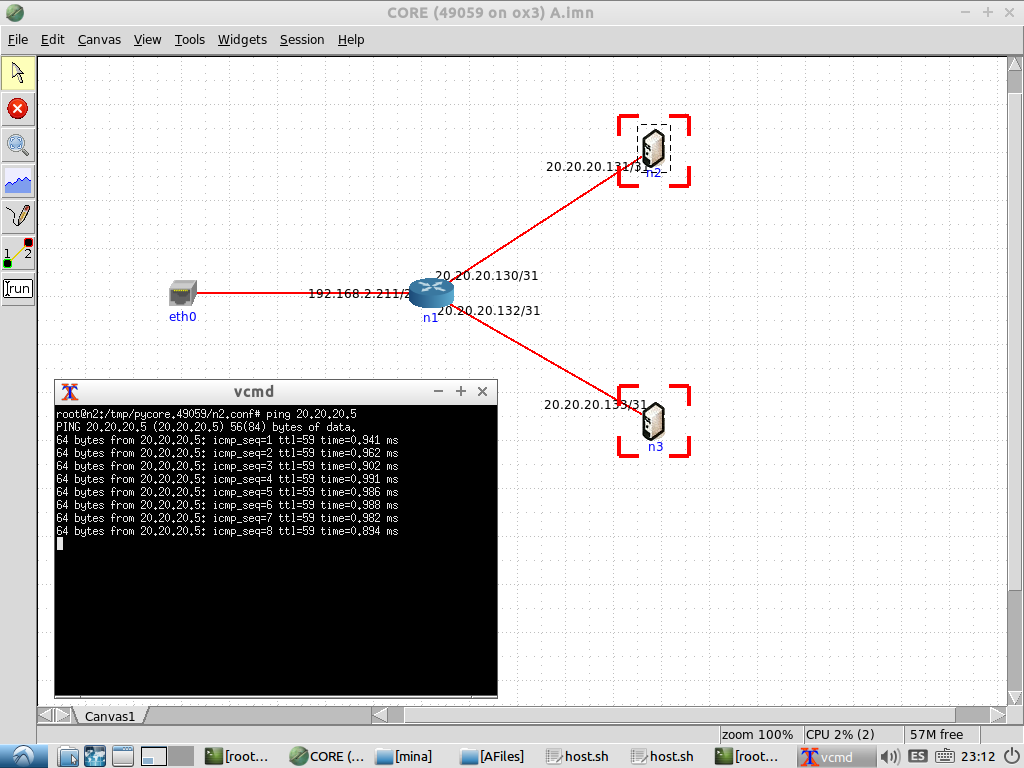
\includegraphics[width=0.6\textwidth]{E1P1/E1P1202020131-2020205}
\caption[Capturas de comando ping H1-Subred A]{Capturas de comando ping H1-Subred A}
\label{fig:LabE1P1CapHost}
\end{figure}

Análogamente se procesan los paquetes asociados a los restantes servicios en el sistema. Para complementar el ejemplo anterior, en la figura \ref{fig:LabE1P1CapsTraf2} se muestra el procesamiento de los paquetes asociados al servicio S3, utilizando el comando ping para generar tr\'afico desde el host 20.20.20.131 en la subred A, al host 20.20.20.67 en la subred B. En la imagen se muestran las capturas de tr\'afico utilizando el comando tcpdump para las interfaces eth1 (cuarto superior izquierdo de la imagen) y nf2 (cuarto superior derecho de la imagen) en el nodo Galois, y las interfaces nf2  
 (cuarto inferior izquierdo) y eth1 (cuarto inferior derecho) en el nodo Poisson.\\


\begin{figure}[ht!] 
\centering    
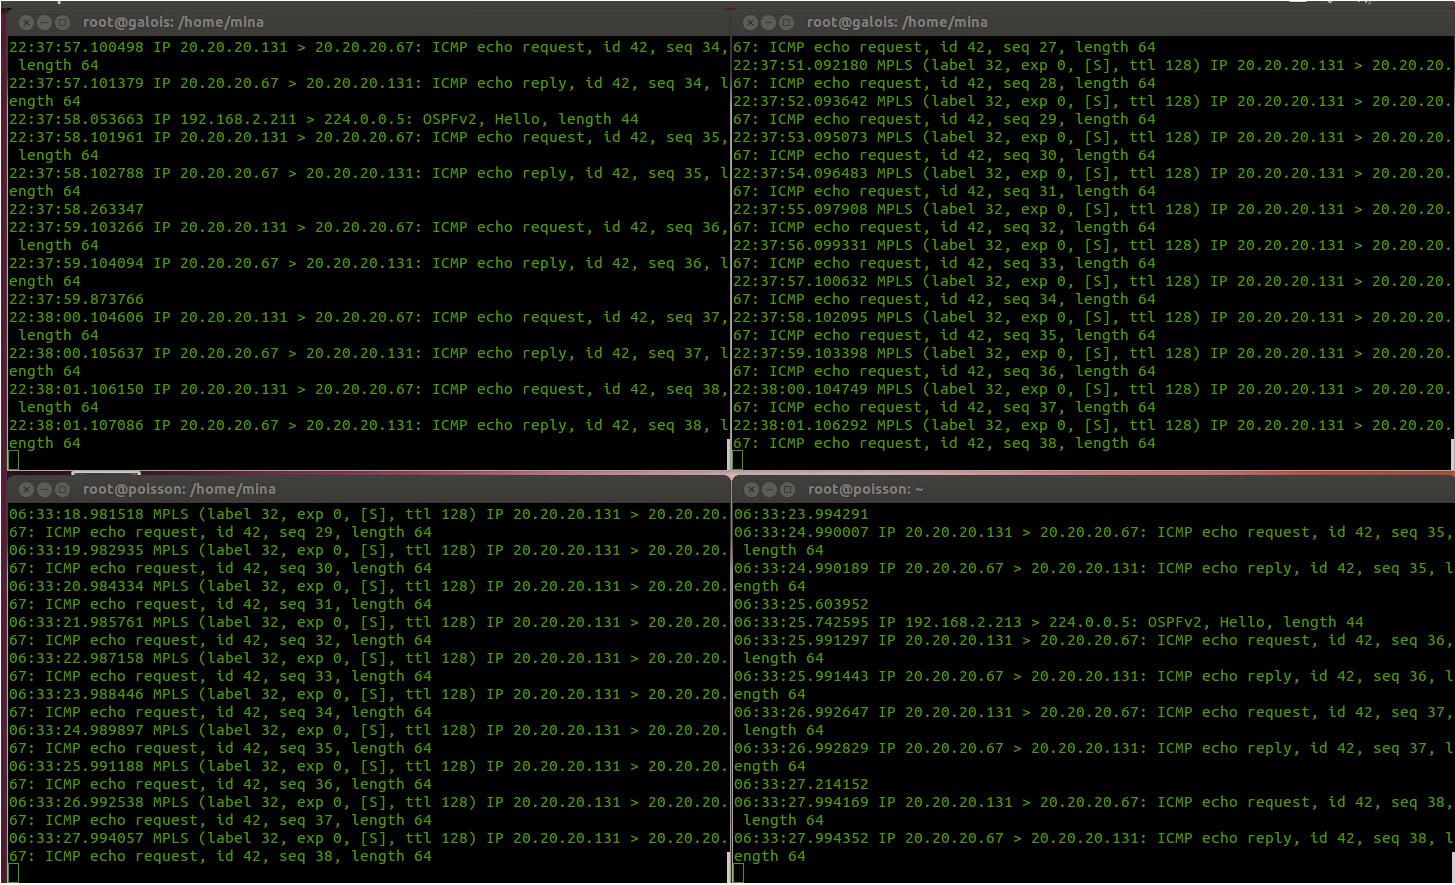
\includegraphics[width=1.0\textwidth]{E1P1/LabE1P1CaputrasTrafico}
\caption[Capturas de tr\'afico con tcpdump - servicio S3]{Capturas de tr\'afico con tcpdump - servicio S3}
\label{fig:LabE1P1CapsTraf2}
\end{figure}

%Sin embargo RAUFlow admite realizar clasificaci\'on de tr\'afico por un conjunto bastante m\'as amplio de atributos. A continuaci\'on se definen una nueva lista de servicios orientados a demostrar la correcta implementaci\'on de esta funcionalidad.

%Cabe destacar que para esta prueba los servicios anteriormente creados son eliminados.

%\begin{table}[h]
%\begin{tabular}{| l | l | l | p{4cm} | p{4cm} |}
%\hline
%Nombre & Ingreso & Egreso & Clasificación & Descripción \\ \hline
%
%\crule[Aquamarine]{0.3cm}{0.3cm} S1 & Galois - eth1 & Oz - eth1 & ip\_src=20.20.20.128/26 ip\_dst=20.20.20.0/26 & Tr\'afico de Subred A a Subred C \\ \hline
%
%\crule[Red]{0.3cm}{0.3cm} S2 & Oz - eth1 & Galois - eth1 & ip\_src=20.20.20.0/26 ip\_dst=20.20.20.128/26 & Tr\'afico de Subred C a Subred A \\ \hline
%
%\crule[ForestGreen]{0.3cm}{0.3cm} S3 & Galois - eth1 & Poisson - eth1 & ip\_src=20.20.20.128/26 ip\_dst=20.20.20.64/26 & Tr\'afico de Subred A a Subred B \\ \hline
%
%\crule[LimeGreen]{0.3cm}{0.3cm} S4 & Poisson - eth1 & Galois - eth1 & ip\_src=20.20.20.64/26 ip\_dst=20.20.20.128/26 & Tr\'afico de Subred B a Subred A \\ \hline
%
%\crule[RoyalPurple]{0.3cm}{0.3cm} S5 & Poisson - eth1 & Oz - eth1 & ip\_src=20.20.20.64/26 ip\_dst=20.20.20.0/26 & Tr\'afico de Subred B a Subred C \\ \hline
%
%\crule[YellowOrange]{0.3cm}{0.3cm} S6 & Oz - eth1 & Poisson - eth1 & ip\_src=20.20.20.0/26 ip\_dst=20.20.20.64/26 & Tr\'afico de Subred C a Subred B \\ \hline
%\end{tabular}
%\vspace{0.3cm}

%\caption[CU1 - Escenario 1, servicios extra]{CU1 - Escenario 1, servicios extra}
%\label{table:TablaFlujos2}
%\end{table}

\section{Escenario 1 - Actualización de Rutas}
\label{appendix6.3}

Para comprobar que el algoritmo de ruteo recaclula correctamente las rutas, se inspeccionan nuevamente las tablas de flujos de cada nodo en el laboratorio (ver figuras \ref{fig:CU1P2DumpFlows1}-\ref{fig:CU1P2DumpFlows4}), comparando los caminos calculados con los caminos te\'oricos.\\

\begin{figure}[h] 
\centering    
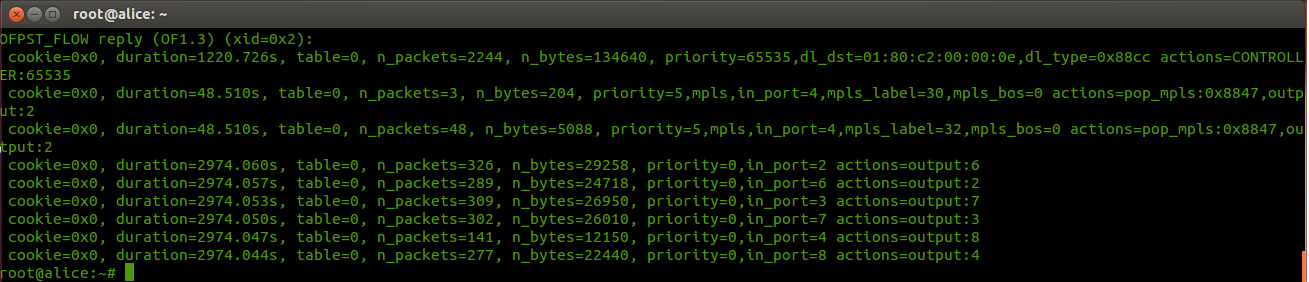
\includegraphics[width=1.0\textwidth]{E1P2/LabE1P2Al}
\caption[Tabla de flujos ovs - Alice]{Tabla de flujos ovs - Alice}
\label{fig:CU1P2DumpFlows1}
\end{figure}

\newpage
\begin{figure}[h] 
\centering    
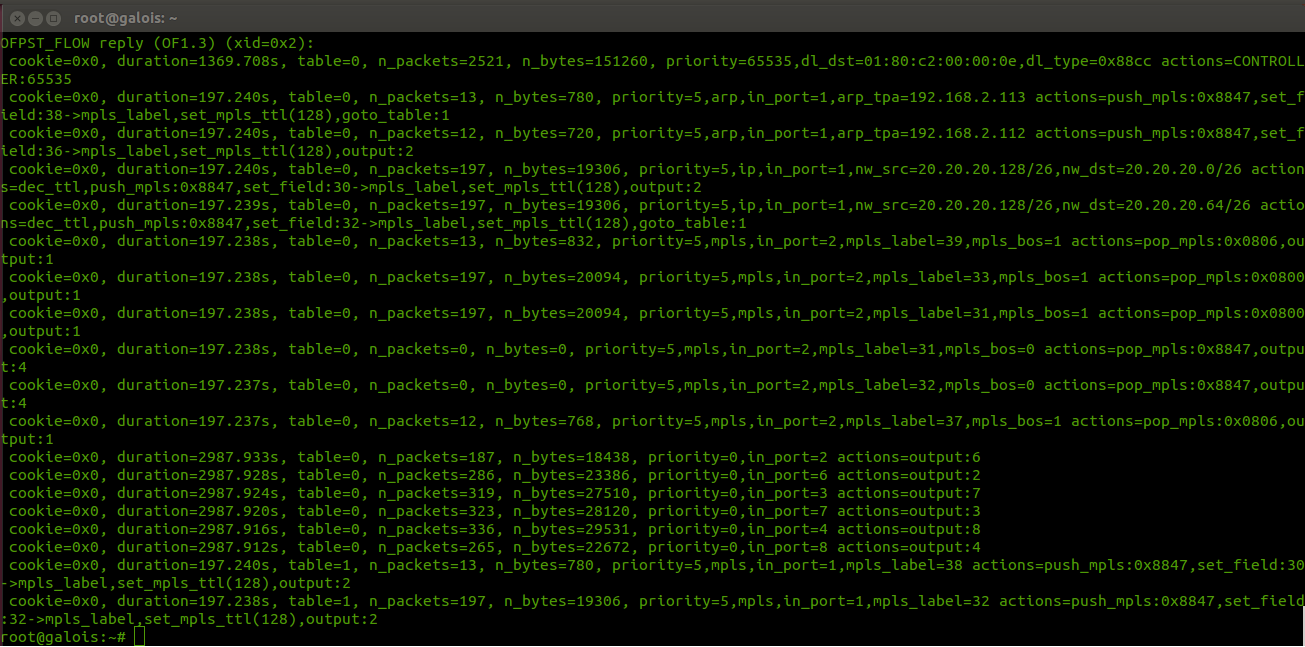
\includegraphics[width=1.0\textwidth]{E1P2/LabE1P2Gal}
\caption[Tabla de flujos ovs - Galois]{Tabla de flujos ovs - Galois}
\label{fig:CU1P2DumpFlows2}
\end{figure}

\begin{figure}[h] 
\centering    
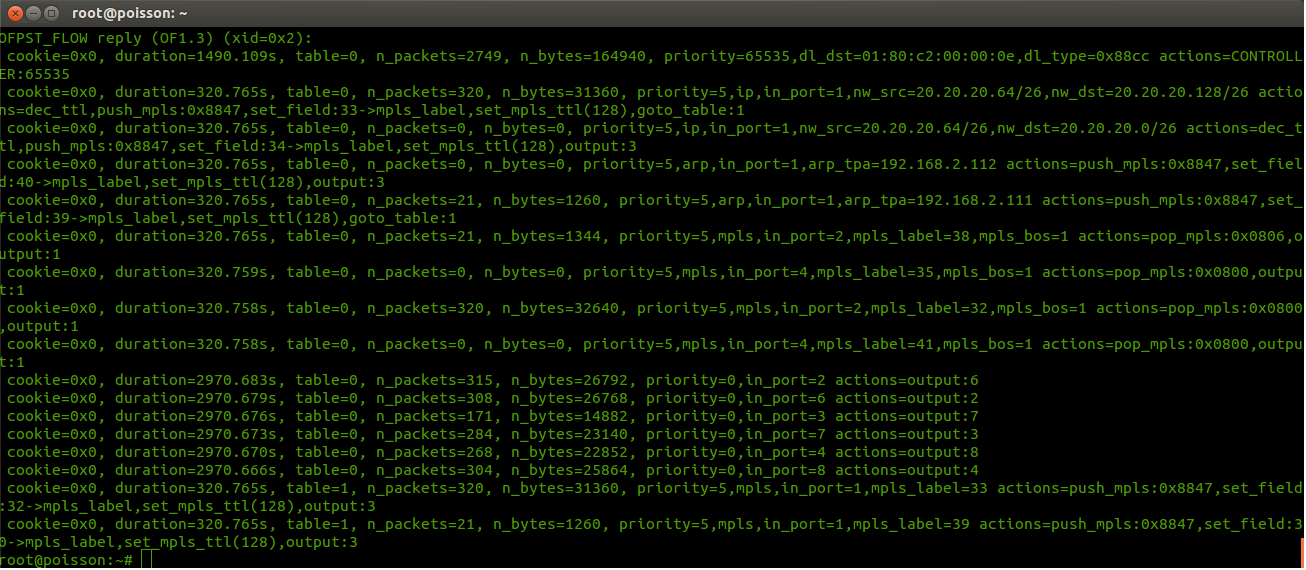
\includegraphics[width=1.0\textwidth]{E1P2/LabE1P2Poi}
\caption[Tabla de flujos ovs - Poisson]{Tabla de flujos ovs - Poisson}
\label{fig:CU1P2DumpFlows3}
\end{figure}

\newpage
\begin{figure}[ht!] 
\centering    
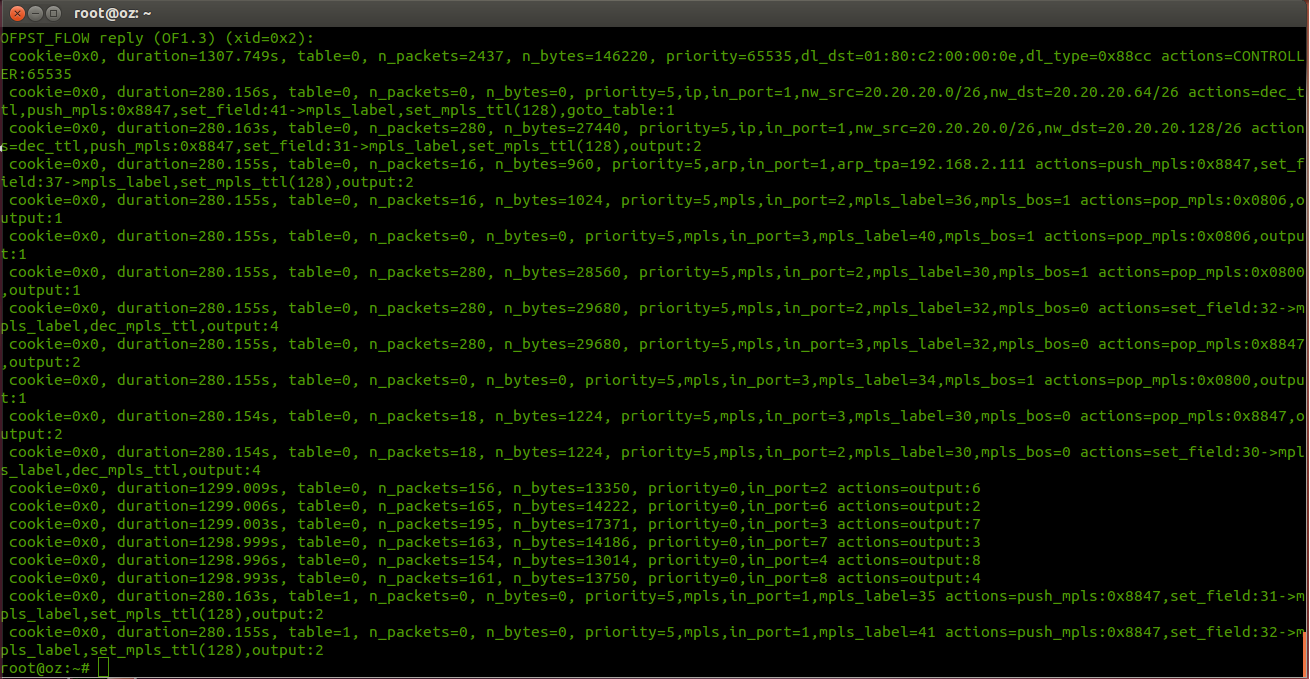
\includegraphics[width=1.0\textwidth]{E1P2/LabE1P2Oz}
\caption[Tabla de flujos ovs - Oz]{Tabla de flujos ovs - Oz}
\label{fig:CU1P2DumpFlows4}
\end{figure}

Tomando como ejemplo la actualizaci\'on del LSP asociado al servicio S3, mientras que en la topolog\'ia original el camino asociado es $<(Galois, nf2)>$, tras la actualizaci\'on de la topolog\'ia el camino correcto puede ser o bien $<(Galois, nf0),(Oz, nf1)>$ o bien \\ $<(Galois, nf0), (Oz, nf2), (Alice, nf0)>$.\\

Al cambiar el camino, los flujos asociados a cada nodo en el camino tambi\'en deben cambiar. En particular como el camino nuevo no comparte ning\'un salto con el camino original, los flujos asociados al camino viejo deben ser eliminados de cada nodo.

Recordando la tabla de flujos original del nodo \textit{Galois} (ver imagen \ref{fig:CU1P1DumpFlows1}), el flujo \ref{fig:Flujo1} es utilizado para procesar y reenviar paquetes al nodo Poisson. En la tabla de flujos actualizada, este flujo es remplazado por el siguiente flujo (ver imagen \ref{fig:CU1P2DumpFlows2}):

\begin{center}
\textit{cookie=0.0, duration=192.239s, table=0, n\_packets=197, n\_bytes=19306, priority=5, \\
ip,in\_port=1, nw\_src=20.20.20.128/26,nw\_dst=20.20.20.64/26 \\
actions=dec\_ttl,push\_mpls:0x8847,set\_field:32->mpls\_label,set\_mpls\_ttl(128), goto\_table:1 \\
cookie=0.0, duration=197.238s, table=0, n\_packets=197, n\_bytes=19306, priority=5, \\
mpls,in\_port=1,mpls\_label=32 actions=push\_mpls:0x8847,set\_fied:32->mpls\_label,set\_mpls\_ttl(128),output:2}
\end{center}

Mediante este par de flujos, se les colocan dos cabezales mpls a los paquetes asociados al servicio, para luego ser reenviados por el puerto numero 2 (interfaz nf0) al nodo \textit{Oz}.\\

Por otra parte en la tabla de flujos del nodo \textit{Oz}, se incorpora el siguiente flujo:

\begin{center}
\textit{cookie=0.0, duration=280.155s, table=0, n\_packets=280, n\_bytes=29680, priority=5, \\
mpls,in\_port=2,mpls\_label=32,mpls\_bos=0 actions=set\_field:30->mpls\_label,dec\_mpls\_ttl,output:4 }
\end{center}

El mismo implementa el cambio de etiqueta mpls en el paquete, y su posterior reenvío por el puerto n\'umero 4 (interfaz nf2).\\

Luego en la tabla de flujos del nodo \textit{Alice} se incorpora el siguiente flujo:

\begin{center}
\textit{cookie=0.0, duration=48.510s, table=0, n\_packets=48, n\_bytes=5088, priority=5, \\
mpls,in\_port=2,mpls\_label=32,mpls\_bos=0 actions=pop\_mpls:0x8847,output:2 }
\end{center}

Este flujo implementa el pop de la etiqueta mpls externa en el penúltimo nodo del LSP (penultimate-pop-hoping). Tras realizar esta acci\'on reenvía el paquete por el puerto n\'umero 2 (interfaz nf0).\\

Finalmente cuando el paquete arriba al nodo \textit{Poisson}, el procesamiento final del paquete, realizado con anterioridad por el flujo \ref{fig:Flujo2} ahora se realiza mediante el siguiente flujo: 

\begin{center}
\textit{cookie=0.0, duration=320.758s, table=0, n\_packets=320, n\_bytes=32740, priority=5, \\
mpls,in\_port=2,mpls\_label=32,mpls\_bos=1 actions=pop\_mpls:0x0800,output:1 }
\end{center}

En la figura \ref{fig:CU1P1DumpFlows1} se muestran capturas tcpdump de las interfaces por las cuales el tr\'afico asociado al servicio S3 atraviesa la red del laboratorio en el nuevo camino calculado.

Enumerando las figuras de izquierda a derecha y de arriba hacia abajo, la primer imagen se corresponde con una captura sobre la interfaz eth1 del nodo Galois, la segunda con la interfaz nf0 del mismo nodo, la tercera con la interfaz nf2 del nodo Oz, la cuarta con la interfaz nf0 del nodo Alice y finalmente la quinta con la interfaz eth1 en el nodo Poisson.

\newpage
\begin{figure}[ht!] 
\centering    
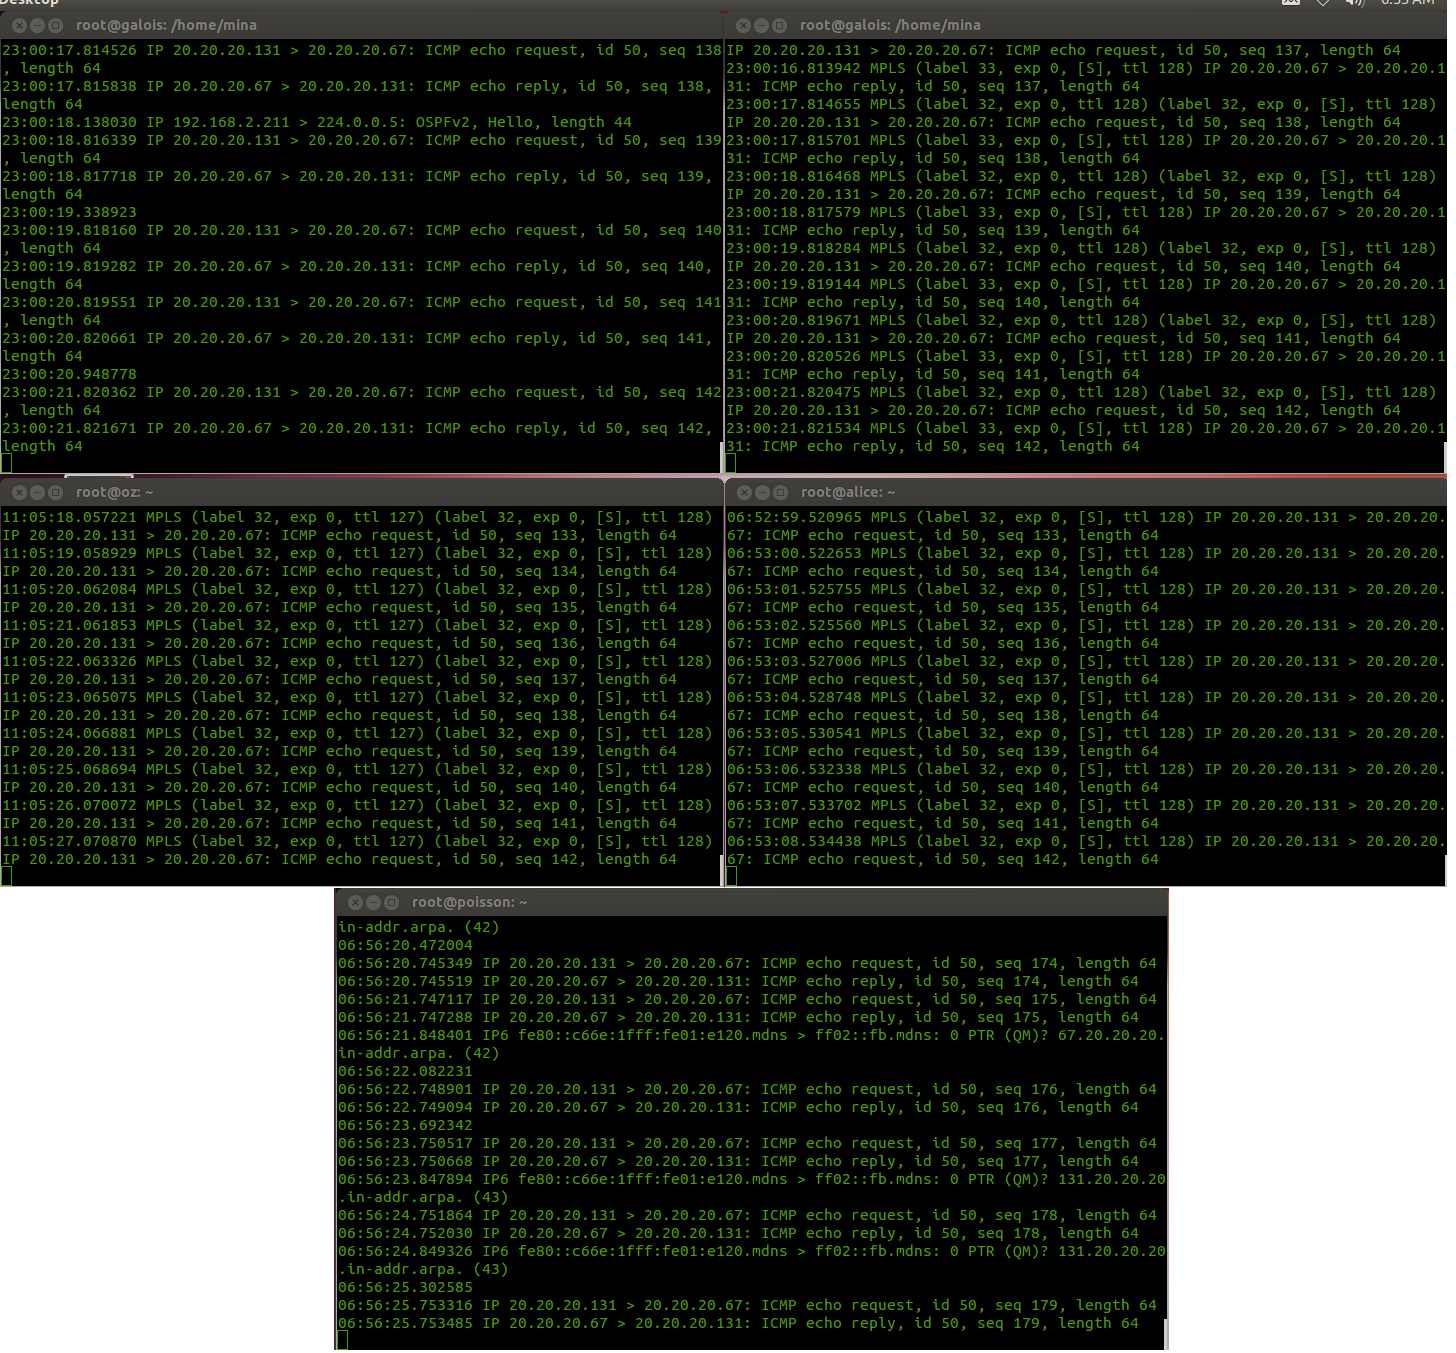
\includegraphics[width=1.0\textwidth]{E1P2/LabE1P2SnapshotTrafico1}
\caption[Capturas de tr\'afico con tcpdump para el servicio S3 tras actualización topol\'ogica]{Capturas de tr\'afico con tcpdump para el servicio S3 tras actualización topol\'ogica}
\label{fig:LabE1P1CapsTraf3}
\end{figure}

Análogamente se puede estudiar la correspondencia entre el camino te\'orico y el camino calculado para el servicio S6.\\
